%% Paper A -- ICT Express letter (template: paper/ICT Express Submission Template_191231.zip, elsarticle 3p twocolumn).
%% Limits: 4 pages incl. references (internal hard limit); abstract 75-100 words; 3-5 keywords, alphabetical.
%% Rewrite 2026-11-25 after the full-data evaluation (fd_v1) and the ChatGPT writing authorisation of 18ddc9e7.
%% Every number: CLAIMS.md (claim -> source). Table: paperA_fd_numbers.py -> table_fd.tex; figures:
%% paperA_fd_figures.py -> figs/fig_fd_system.pdf, figs/fig_fd_results.pdf. Previous method letter: git 1225e287.
\documentclass[final,3p,times,twocolumn]{elsarticle}
\usepackage{graphicx, amsmath, amssymb, booktabs, xcolor, siunitx}
\usepackage[utf8]{inputenc}
\usepackage[english]{babel}
\usepackage{hyperref}
\hypersetup{colorlinks=true, linkcolor=black, filecolor=black, urlcolor=cyan, citecolor=black}
\usepackage{caption}
\captionsetup{justification=raggedright, singlelinecheck=false}
\captionsetup[table]{labelformat=simple, labelsep=newline}
\captionsetup[figure]{labelformat=simple, labelsep=period}
\newcommand{\todo}[1]{\textcolor{red}{[TODO: #1]}}

\journal{ICT Express}

\begin{document}
\begin{frontmatter}

\title{Uncertainty-aware mode selection for multi-UAV semantic image offloading}

\author{\todo{Author 1}\corref{cor1}}
\ead{\todo{email}}
\author{\todo{Author 2}}
\ead{\todo{email}}
\address{\todo{Department, Organization, City, Country}}
\cortext[cor1]{Corresponding author}

\begin{abstract}
Predictive selection of image transmission modes relies on rate models that are inaccurate under link adaptation (LA).
We evaluate a selective model-predictive control (MPC) layer that may override an incumbent mode policy and screens
each switch against the tracked rate-prediction error. In a multi-UAV simulator with block-level LA and 27,600
episodes on VisDrone images, unguarded nominal MPC underperforms a tuned heuristic, whereas the uncertainty-aware
layer improves return in the reference and five of six other settings and over three reinforcement-learning
incumbents, mainly through its uncertainty band. ACK calibration helps only conditionally, and return gains do not
imply higher detection recall.
\end{abstract}

\begin{keyword}
Link adaptation \sep Model predictive control \sep Semantic communication \sep Uncertainty \sep Unmanned aerial
vehicles
\end{keyword}

\end{frontmatter}

\begin{figure*}[t]
\centering
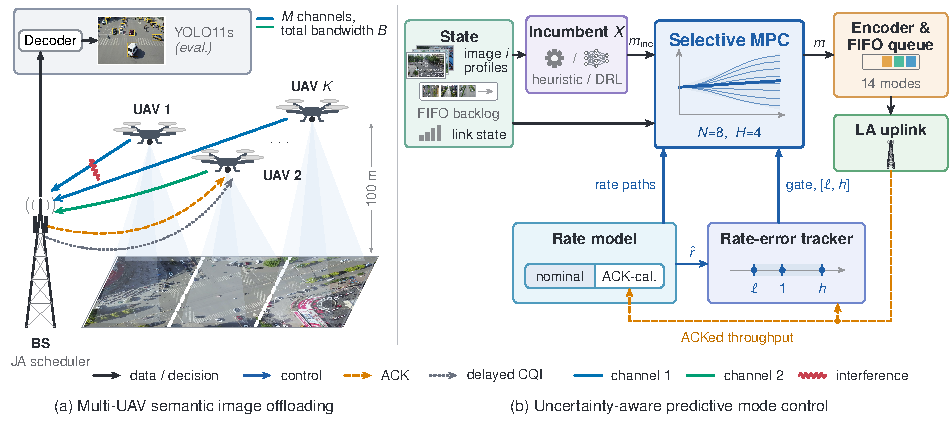
\includegraphics[width=0.95\textwidth]{figs/fig_fd_system.pdf}
\caption{System and controller. The selective MPC may override the incumbent's mode; the rate model supplies rate
paths, and the error tracker supplies the cold-start gate and the uncertainty band $[\ell,h]$.}
\label{fig:system}
\end{figure*}

\section{Introduction}\label{sec:intro}
UAVs surveying an area offload many images to a base station (BS) under deadlines and limited bandwidth. Semantic
communication adapts each image's representation (compression level, learned or generative codec), often chosen by
deep reinforcement learning together with radio resources and trajectories \cite{huang2025,zhao2026}, with rates from
capacity formulas, whereas practical link adaptation (LA) selects the modulation and coding scheme (MCS) from delayed
channel reports, corrects it with an outer loop and retransmits failed blocks \cite{3gpp36213}. Model-predictive control (MPC) with error-discounted throughput prediction is
established in video streaming \cite{yin2015}, and switching between a learned policy and a fallback according to
uncertainty has been proposed for learning-augmented systems \cite{rotman2020}. A second issue is the objective: the
communication utility that such controllers maximise rewards quality margins, delay and mission time, whereas the
receiver's purpose is a task such as object detection.

Rather than a new MPC algorithm, this letter contributes (C1) a multi-UAV image-offloading framework combining
adaptive transmission modes, block-level LA and a selective MPC layer with uncertainty-aware screening on top of any
incumbent mode policy; (C2) a largely pre-registered evaluation separating the uncertainty band, a cold-start gate,
ACK calibration and the planning horizon across network settings and incumbents; and (C3) an analysis of the
trade-offs among communication return, detection recall and decision time, with a post-hoc return decomposition.

\section{System model and problem formulation}\label{sec:model}
$K$ UAVs survey disjoint sectors at \SI{100}{m} with paced flight and offload each image (52 per UAV) to a BS over
$M$ channels sharing $B$ at \SI{2.4}{GHz} ($K{=}5$, $M{=}2$, $B{=}\SI{1}{MHz}$ by default), with the channel of
\cite{alhourani2014}, Rician fading and the energy model of \cite{zeng2019}. In every \SI{1}{s} slot a
joint-assignment (JA) scheduler enumerates the $(M{+}1)^K$ channel assignments. Each \SI{0.1}{s} block uses one LTE
CQI-table MCS \cite{3gpp36213}, chosen from an SNR report delayed by two blocks with \SI{1}{dB} error, the BS's
knowledge of co-scheduled UAVs and an outer-loop offset (10\% block-error target); block errors follow a logistic
curve at the worst SINR in the block, only acknowledged (ACKed) bits count, failed blocks are retransmitted until the
deadline, and co-channel UAVs interfere for the whole slot. All LA parameters are assumptions.

Images are VisDrone frames \cite{visdrone}, each sent in one of 14 modes (AVIF, a learned codec \cite{minnen2018} and
JPEG2000 at several qualities, a thumbnail, three generative modes) with measured payload, PSNR and encoding time.
Image $i$ has a deadline $D_i^{\max}\sim U(4,12)$\,s and a quality floor $Q_i^{\min}\sim U(22,30)$\,dB; delivered with
PSNR $q_i$ and delay $D_i$ it obtains
\begin{multline}\label{eq:u}
u_i = 0.5\,\mathrm{clip}\!\left(\tfrac{q_i-Q_i^{\min}}{15},-1,1\right) + 0.5\,\tfrac{\max(D_i^{\max}-D_i,0)}{D_i^{\max}}\\
- \mathbf{1}\!\left[q_i<Q_i^{\min} \lor D_i>D_i^{\max}\right],
\end{multline}
and a dropped image obtains $u_i=-1$. Mode selection maximises the episode return
\begin{equation}\label{eq:J}
J=\textstyle\sum_i u_i-0.02\,E-0.3\sum_k T_k,
\end{equation}
with the UAV energy $E$ in kJ and the mission time $T_k$ of UAV $k$ in seconds (a UAV stays active until its queue is
empty). When an image's mode is due, an incumbent policy $X$ proposes $m_{\mathrm{inc}}$, which the layer below may
override. Detection recall, the share of ground-truth objects found by a YOLO11s detector \cite{yolo11}
(IoU $\ge 0.5$) in images delivered on time with $q_i\ge Q_i^{\min}$, is evaluated but never optimised.

\begin{figure*}[t]
\centering
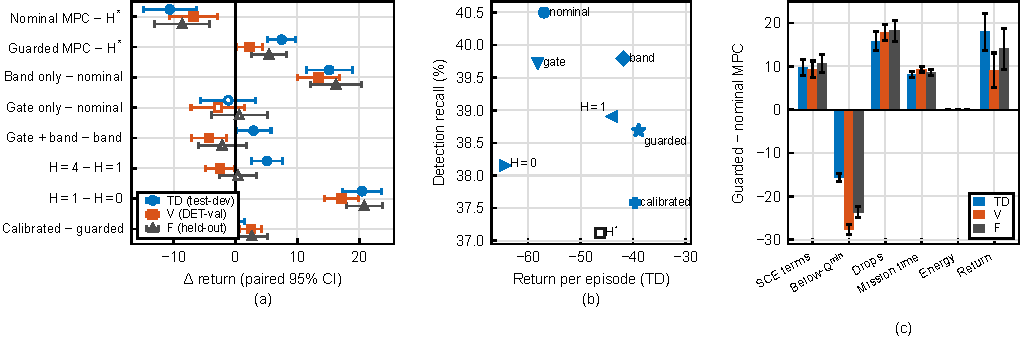
\includegraphics[width=\textwidth]{figs/fig_fd_results.pdf}
\caption{Reference setting, ablation seeds. (a) Paired return differences (95\% CIs; hollow: CI includes 0).
(b) Return and recall per arm on TD. (c) Post-hoc decomposition of guarded minus nominal MPC into the terms of
\eqref{eq:u}--\eqref{eq:J} (SCE: quality and deadline terms).}
\label{fig:results}
\end{figure*}

\begin{table*}[t]
\caption{Paired differences on TD (100 seeds). $^\dagger$ Holm-rejected pre-registered test; $^*$ CI excludes 0
(recall, in points: seed-level and video-cluster CIs; $^\circ$ seed-level only). Timing of the guarded MPC: sequential
per-slot p99 (ms) / slots over \SI{50}{ms}, sequential / parallel per-UAV (\%). $^a$ Ablation seeds.}
\label{tab:main}
\centering
\small
% generated by swarmbridge/experiments/uav_semcom/paperA_fd_numbers.py from stored results; do not edit
\begin{tabular}{@{}lccccc@{}}
\toprule
 & \multicolumn{2}{c}{Guarded MPC $-$ base} & \multicolumn{2}{c}{Calibrated $-$ guarded MPC} & Timing \\
\cmidrule(lr){2-3}\cmidrule(lr){4-5}
Setting & $\Delta$return [95\% CI] & $\Delta$recall & $\Delta$return [95\% CI] & $\Delta$recall & ms / \% / \% \\
\midrule
\multicolumn{6}{@{}l}{\emph{Base: tuned heuristic $H^*$ (re-tuned per setting)}} \\
$K{=}5$, $M{=}2$, 1 MHz (ref.)$^a$ & +7.4$^*$ {\scriptsize[+5.1, +9.8]} & +1.6$^*$ & $-$0.7 {\scriptsize[$-$2.9, +1.4]} & $-$1.1$^*$ & 160 / 63 / 0.1 \\
$K{=}3$, $M{=}2$ & +0.6 {\scriptsize[$-$0.8, +2.0]} & $-$0.1 & +1.3$^*$ {\scriptsize[+0.1, +2.6]} & $-$0.4$^*$ & 110 / 44 / 0.0 \\
$K{=}7$, $M{=}2$ & +6.8$^\dagger$ {\scriptsize[+3.4, +10.2]} & +1.4$^*$ & +1.3 {\scriptsize[$-$2.5, +5.2]} & $-$0.6$^*$ & 220 / 73 / 30.7 \\
$K{=}5$, $M{=}3$ & +5.2$^\dagger$ {\scriptsize[+2.8, +7.6]} & $-$0.4$^\circ$ & +2.8$^\dagger$ {\scriptsize[+1.0, +4.6]} & $-$0.6$^*$ & 166 / 66 / 3.7 \\
$K{=}5$, $M{=}4$ & +2.9$^\dagger$ {\scriptsize[+1.8, +4.1]} & $-$0.2$^\circ$ & +1.6$^\dagger$ {\scriptsize[+0.5, +2.8]} & $-$0.6$^*$ & 189 / 72 / 41.1 \\
$B{=}0.5$ MHz & +7.4$^\dagger$ {\scriptsize[+5.5, +9.4]} & +2.3$^*$ & +0.2 {\scriptsize[$-$1.7, +2.1]} & $-$0.8$^*$ & 157 / 62 / 0.0 \\
$B{=}2$ MHz & +4.9$^\dagger$ {\scriptsize[+2.8, +7.0]} & +1.2$^*$ & +2.1 {\scriptsize[$-$0.5, +4.7]} & $-$1.0$^*$ & 177 / 58 / 0.0 \\
\midrule
\multicolumn{6}{@{}l}{\emph{Base: learned incumbent $X$ alone ($K{=}5$, $M{=}2$, 1 MHz)}} \\
PPO & +7.4$^\dagger$ {\scriptsize[+6.0, +8.8]} & +2.4$^*$ & +3.1$^\dagger$ {\scriptsize[+1.6, +4.7]} & $-$0.4$^*$ & 173 / 65 / 0.1 \\
QR-DQN & +19.0$^\dagger$ {\scriptsize[+17.0, +21.0]} & +5.2$^*$ & +4.7$^\dagger$ {\scriptsize[+3.0, +6.3]} & $-$0.4$^*$ & 158 / 62 / 0.0 \\
Discrete SAC & +25.7$^\dagger$ {\scriptsize[+23.8, +27.7]} & +7.0$^*$ & +6.0$^\dagger$ {\scriptsize[+4.2, +7.8]} & $-$0.7$^*$ & 160 / 63 / 0.0 \\
\bottomrule
\end{tabular}

\end{table*}

\section{Uncertainty-aware mode selection}\label{sec:method}
\emph{Rate models.} The \emph{nominal} model applies the LA rate mapping (CQI rate times one minus the block-error
target) to fading samples of the statistical channel model, without report delay, outer loop, retransmissions or
interference. The \emph{ACK-calibrated} model stores each transmitting UAV's ACKed bits per second of airtime after
every slot in the \SI{2}{dB} bin of its expected SNR, pooled over UAVs, and samples rate paths i.i.d.\ per slot from
the bin (neighbouring bins are merged until \SI{20}{s} of data exist). Both restart in every episode.

\emph{Error tracker, gate and band.} The ratio of realised to predicted mean rate of every slot is added to the same
SNR bins. Until \SI{20}{s} of airtime is observed, planning is gated off and $m_{\mathrm{inc}}$ is kept; then the
relative bias $b$ and the standard error $\sigma$ of the ratio give the band $\ell=\max(\min(1,1{+}b)-2\sigma,0.05)$,
$h=\max(1,1{+}b)+2\sigma$.

\emph{Selective MPC} (Fig.~\ref{fig:system}). A screen evaluates the 14 modes one image ahead on rate paths scaled by
1 and by $\ell$; the best mode at each scale becomes a candidate, and planning continues only if a candidate beats
$m_{\mathrm{inc}}$. The full plan uses $N{=}8$ rate paths over \SI{40}{s} and simulates the UAV's encoder and
transmitter queues for the current, the queued and the next $H{=}4$ images (modes of later images chosen greedily). The
MPC switches only if the mean paired gain exceeds one standard error and stays positive with all paths scaled by
$\ell$ and by $h$. A \SI{50}{ms} budget per decision is checked before each stage; otherwise $m_{\mathrm{inc}}$ is
kept. With the nominal model the layer is the \emph{guarded MPC}, with the calibrated model the \emph{calibrated MPC};
the planner without gate and band ($\ell{=}h{=}1$) is the \emph{nominal MPC}. Ablations remove the gate, the band or
anticipated images ($H{=}1$, $H{=}0$).

\section{Experimental setup}\label{sec:setup}
Pools are sequence-disjoint subsets of VisDrone2019-DET with at most 30 frames per sequence: training (1,523 frames)
and validation (374) from DET-train, and test pools TD (test-dev, 582 frames, 61 sequences; primary), F (168 frames,
18 DET-train sequences withheld from detector training) and V (DET-val, 548). V and 49 TD sequences were used in
earlier development, and F selected the detector checkpoint; recall is reported on test pools only. Incumbents are
$H^*$, the best of 22 fixed or backlog-budget rules on training seeds (AVIF-20 in the reference setting, re-tuned per
setting), and PPO \cite{schulman2017}, QR-DQN \cite{dabney2018} and Discrete SAC \cite{christodoulou2019}, each with
three training seeds of 2M decisions, checkpoints chosen on validation and fixed hyper-parameters. Besides the
reference we vary $K\in\{3,7\}$, $M\in\{3,4\}$ and $B\in\{0.5,2\}$\,MHz. All arms of a pool share 100 environment seeds;
we report paired differences with 95\% $t$-confidence intervals (CIs), averaging learned incumbents over training
seeds, and add a video-cluster bootstrap for recall. Confirmatory hypotheses were pre-registered and
Holm-corrected within families (reference 2, ablation 4, network settings 12, learned incumbents 6); 27,600 episodes
were run. The return decomposition and the PPO-versus-$H^*$ comparison with calibrated MPC are post-hoc. Protocols,
code and results: \url{https://github.com/vutl/SwarmBridge}.

\section{Results and discussion}\label{sec:results}
\textbf{F1: nominal predictive control can underperform the incumbent.} The nominal MPC trails $H^*$ by $-10.6$
$[-14.8,-6.4]$ on TD ($-6.8$ on V, $-8.6$ on F; Fig.~\ref{fig:results}a). The nominal model over-predicts the
realised rate (median relative bias $-0.38$, as tracked in the guarded arm); the planner switches modes 180 times per
episode and drops 8.1\% of the images ($H^*$:
2.1\%).

\textbf{F2: uncertainty-aware screening, mainly the band, makes MPC useful.} In the pre-registered reference test the
calibrated MPC improves on $H^*$ by $+7.3$ $[+5.0,+9.5]$; the guarded MPC gains $+7.4$ on the ablation seeds
(Table~\ref{tab:main}). The band alone recovers $+15.2$ over the nominal MPC on TD (Holm; $+13.4$ on V, $+16.2$ on F),
the gate alone has no detected effect ($-1.2$), and adding the gate to the band is inconsistent ($+2.9$, $-4.3$,
$-2.1$ on TD, V, F). One anticipated image matters ($H{=}1$ vs.\ $H{=}0$: $+17$ to $+21$); four do not
replicate a further gain ($+5.1$ on TD, Holm; $-2.5$ on V; $+0.4$ on F). The guarded MPC improves on the re-tuned
$H^*$ in five of six other settings (Holm; no detected difference at $K{=}3$) and improves all three learned
incumbents.

\textbf{F3: calibration is conditional, and return is not recall.} Within the guarded design, ACK calibration shows no
detected effect in the pre-registered reference test ($-0.1$ $[-2.0,+1.8]$; $+2.5$ and $+2.6$ in the V and F ablation
replications), and improves return at $M{=}3$ and $M{=}4$ (Holm) and for all learned incumbents. No learned
incumbent showed a detected return advantage over $H^*$ (PPO $-3.0$ $[-4.9,-1.0]$, QR-DQN $-22.5$, Discrete SAC
$-34.1$); with calibrated MPC on both, PPO differs by $+0.3$ $[-1.6,+2.1]$ (not evidence of equivalence).

Recall ranks the arms differently (Fig.~\ref{fig:results}b): the nominal MPC has the highest recall (40.5\%; guarded
38.7\%, calibrated 37.6\%, $H^*$ 37.1\%) although its return is 18.1 below the guarded MPC, and calibration lowers
recall in every row of Table~\ref{tab:main} ($-0.4$ to $-1.1$ points). The post-hoc decomposition
(Fig.~\ref{fig:results}c) shows that the guarded MPC sends smaller payloads per compliant image than the nominal MPC
(194 vs.\ 303\,kbit): it drops 15.8 fewer images but delivers 15.7 more below
$Q^{\min}$, which \eqref{eq:u} penalises equally, so its $+18.1$ return gain comes from the SCE terms ($+9.7$; mean
delay \SI{1.2}{s} shorter) and from missions shorter by \SI{5.4}{s} per UAV ($+8.1$). Its recall is 1.8 points lower:
1.2 from a lower detection yield on images compliant under both arms and 0.6 from a different compliant set. Of 53
decomposed contrasts, 44 had a positive mean return difference and 41 of these sent smaller payloads (exceptions: the
guarded MPC versus $H^*$ in three pools); a PPO checkpoint trained on earlier data sends larger payloads and has
higher recall ($+3.1$ points) but lower return ($-4.9$) than $H^*$. With the weights of \eqref{eq:J}, return rewards
fast delivery and short missions but not detections beyond the quality floor, so controllers that raised return often
did so by sending fewer bits.

\textbf{Decision time.} The simulator runs a slot's mode decisions sequentially without charging their duration. For
every planner with $H{\ge}1$ the per-slot 99th percentile is 103--229\,ms and 42--82\% of slots exceed \SI{50}{ms};
with parallel per-UAV decisions at most 4.1\% do for $K{\le}5$, $M{\le}3$, but 31\% at $K{=}7$ and 41\% at $M{=}4$
(guarded MPC, TD), where the JA scheduler alone takes about 30\,ms. $H{=}0$ fits (16\,ms) but plans worst. Because of the wall-clock budget,
MPC results are not bit-reproducible.

\section{Conclusions}\label{sec:conclusion}
Screening mode switches against the tracked rate-prediction error, chiefly through the uncertainty band, turned
predictive mode selection from worse than a tuned heuristic into better than it in most tested settings; ACK
calibration helped only in some, and communication return was not a proxy for detection recall. Limitations: one
simulator with assumed LA parameters and objective weights, one detector, a post-hoc mechanism analysis, uncharged
decision time and an exhaustive scheduler.

\section*{Acknowledgments}
\todo{funding}

\section*{Conflict of interest}
The authors declare that there is no conflict of interest in this paper.

\begin{thebibliography}{99}
\bibitem{huang2025} C. Huang, X. Chen, G. Chen, et al., Deep reinforcement learning-based
resource allocation for hybrid bit and generative semantic communications in space-air-ground integrated networks,
IEEE J. Sel. Areas Commun. 43 (12) (2025) 3942--3954.
\bibitem{zhao2026} A. Zhao, M. Sun, X. Xu, et al., Adaptive task-oriented
semantic communication for UAVs with joint trajectory and resource optimization, IEEE Trans. Netw. Sci. Eng. 13 (2026)
11622--11642.
\bibitem{3gpp36213} 3GPP, Evolved Universal Terrestrial Radio Access (E-UTRA); Physical layer procedures, TS 36.213,
Release 8.
\bibitem{yin2015} X. Yin, A. Jindal, V. Sekar, B. Sinopoli, A control-theoretic approach for dynamic adaptive video
streaming over HTTP, in: Proc. ACM SIGCOMM, 2015, pp. 325--338.
\bibitem{rotman2020} N. H. Rotman, M. Schapira, A. Tamar, Online safety assurance for learning-augmented systems, in:
Proc. ACM HotNets, 2020, pp. 88--95.
\bibitem{alhourani2014} A. Al-Hourani, S. Kandeepan, S. Lardner, Optimal LAP altitude for maximum coverage, IEEE
Wireless Commun. Lett. 3 (6) (2014) 569--572.
\bibitem{zeng2019} Y. Zeng, J. Xu, R. Zhang, Energy minimization for wireless communication with rotary-wing UAV, IEEE
Trans. Wireless Commun. 18 (4) (2019) 2329--2345.
\bibitem{visdrone} P. Zhu, L. Wen, D. Du, et al., Detection and tracking meet drones
challenge, IEEE Trans. Pattern Anal. Mach. Intell. 44 (11) (2022) 7380--7399.
\bibitem{minnen2018} D. Minnen, J. Ball\'e, G. Toderici, Joint autoregressive and hierarchical priors for learned image
compression, in: Adv. Neural Inf. Process. Syst. (NeurIPS), 2018.
\bibitem{yolo11} G. Jocher, J. Qiu, Ultralytics YOLO11, software, 2024.
\bibitem{schulman2017} J. Schulman, F. Wolski, P. Dhariwal, et al., Proximal policy optimization
algorithms, arXiv:1707.06347, 2017.
\bibitem{dabney2018} W. Dabney, M. Rowland, M. G. Bellemare, R. Munos, Distributional reinforcement learning with
quantile regression, in: Proc. AAAI Conf. Artif. Intell., 2018.
\bibitem{christodoulou2019} P. Christodoulou, Soft actor-critic for discrete action settings, arXiv:1910.07207, 2019.
\end{thebibliography}
\end{document}
